\section{Errori nel calcolo di funzioni non razionali}
Nel caso in cui si abbia a che fare con una \textbf{funzione non razionale} dobbiamo, prima di
procedere al calcolo in macchina, approssimarla con una funzione razionale. Dobbiamo trovare una
funzione $h$ che approssima $f$, la quale introduce un nuovo tipo di errore, detto
\textbf{errore analitico}
\[ \ean = \frac{h(x) - f(x)}{f(x)} \]
Un possibile modo di approssimare la funzione $f$ è tramite lo sviluppo di Taylor arrestato ad un certo ordine.

In questo corso non trattiamo l'errore analitico ma siamo comunque interessati all'analisi dell'errore inerente
e algoritmico di funzioni non razionali.

\begin{example}
	Studiamo il condizionamento della funzione
	\[ f(x) = \frac{e^x - 1}{x} \]
	per $x \to 0^+$. Come sappiamo l'errore inerente, in un'analisi al primo ordine, equivale a
	\[ \ein = \frac{f'(x)}{f(x)} \epsilon_x x \]
	mentre l'errore di rappresentazione sul dato iniziale equivale a
	\[ \epsilon_x = \frac{\tx - x}{x} \]
	con $|\epsilon_x| \leq u$. Per prima cosa dobbiamo calcolare la derivata della funzione $f$
	\[ f'(x) = \frac{x e^x - 1 (e^x - 1)}{x^2} = \frac{x e^x - e^x + 1}{x^2} \]
	Possiamo ora calcolare il coefficienti di amplificazione
	\[
		c_x = \frac{f'(x)}{f(x)} x =
		\frac{x e^x - e^x + 1}{x^2} \frac{x}{e^x - 1} x =
		\frac{x e^x - e^x + 1}{e^x - 1}
	\]
	Il limite per $x \to 0^+$, come possiamo notare, è un caso di indeterminazione
	\[ \lim_{x \to 0^+} \frac{x e^x - e^x + 1}{e^x - 1} = \frac{0}{0} \]
	risolvibile con il teorema di de l'H\^ospital calcolando il limite
	\[ \lim_{x \to 0^+} \frac{e^x + x e^x - e^x}{e^x} = \lim_{x \to 0^+} x = 0 \]
	Concludiamo quindi che il problema per $x \to 0^+$ è perfettamente ben condizionato.
\end{example}

\begin{example}
	Calcoliamo l'errore algoritmico della funzione
	\[ f(x) = \frac{e^x - 1}{x} \]
	assumendo di avere a disposizione una funzione di macchina \verb|Exp| tale che
	\[ \text{Exp} (x) = e^x (1 + \epsilon) \]
	con $|\epsilon| \leq u$. La funzione effettivamente calcolata in macchina è quindi
	\[
		g(x) = (\text{Exp} (x) \ominus 1) \oslash x =
		\frac{(e^x (1 + \epsilon_1) - 1) (1 + \epsilon_2)}{x} (1 + \epsilon_3)
	\]
	Da qui possiamo procedere con un'analisi in avanti dell'errore
	\begin{center}
		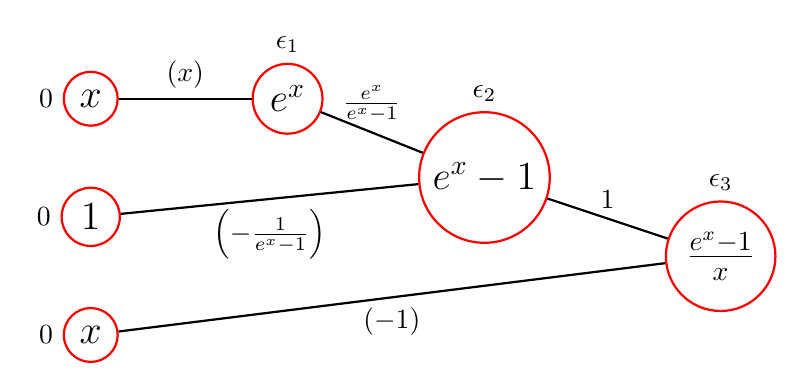
\begin{tikzpicture}[mynode/.style={draw=red, thick, circle, font=\Large}]
			\node[mynode, label=left:$0$] at (0, 1.5) (x1) {$x$};
			\node[mynode, label=left:$0$] at (0, 0) (1) {$1$};
			\node[mynode, label=left:$0$] at (0, -1.5) (x2) {$x$};

			\node[mynode, label=above:$\epsilon_1$] at (2.5, 1.5) (e^x) {$e^x$};
			\node[mynode, label=above:$\epsilon_2$] at (5, 0.5) (e^x-1) {$e^x - 1$};
			\node[mynode, label=above:$\epsilon_3$] at (8, -0.5) (e^x-1/x) {$\frac{e^x-1}{x}$};

			\path
			(x1) edge[thick] node[above, black] {$(x)$} (e^x)
			(e^x) edge[thick] node[above, black] {$\frac{e^x}{e^x-1}$} (e^x-1)
			(1) edge[thick] node[below, black] {$\left( -\frac{1}{e^x-1} \right)$} (e^x-1)
			(e^x-1) edge[thick] node[above, black] {$1$} (e^x-1/x)
			(x2) edge[thick] node[below, black] {$(-1)$} (e^x-1/x);
		\end{tikzpicture}
	\end{center}
	Dalla quale otteniamo
	\begin{align*}
		\ealg =   & \epsilon_3 + 1 \left( \epsilon_2 + \frac{e^x}{e^x - 1} \epsilon_1 \right)              \\
		|\ealg| = & \left| \epsilon_3 + 1 \left( \epsilon_2 + \frac{e^x}{e^x-1} \epsilon_1 \right) \right| \\
		\leq      & |\epsilon_3| + |\epsilon_2| + \left| \frac{e^x}{e^x-1} \right| \left|\epsilon_1\right| \\
		\leq      & 2u + \frac{e^x}{|e^x - 1|} u
	\end{align*}
	Concludiamo quindi che l'algoritmo è numericamente instabile quando $x$ tende a 0 da destra poiché
	\[ \lim_{x \to 0^+} \frac{e^x}{|e^x-1|} = +\infty \]
\end{example}

\begin{example}
	Consideriamo ora l'ultimo caso in cui introduciamo un cambio di variabile
	\[ y = e^x \]
	e siamo interessati a valutare la stabilità di un algoritmo equivalente a quello visto negli esercizi appena
	svolti, ossia
	\[ g(y) = \frac{y - 1}{\ln (y)} \]
	Assumiamo di avere a disposizione una funzione di macchina \verb|Ln| per il calcolo del logaritmo naturale
	tale che
	\[ \text{Ln}(y) = \ln (y) (1 + \epsilon_1) \]
	con $|\epsilon_1| \leq u|$. Procediamo con un'analisi in avanti dell'errore algoritmico
	\begin{center}
		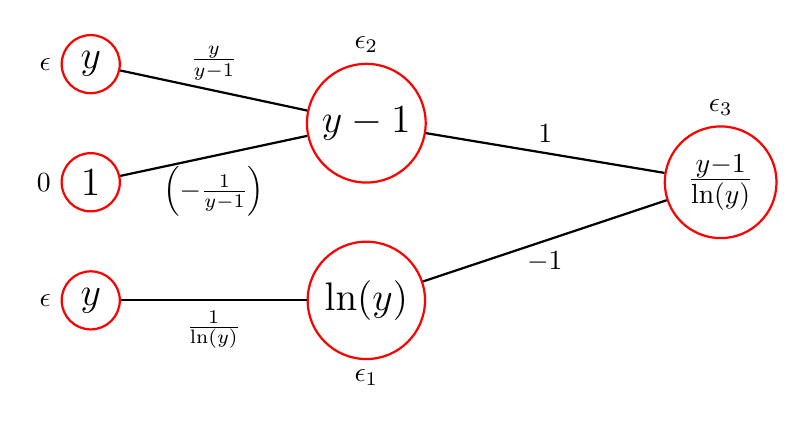
\begin{tikzpicture}[mynode/.style={draw=red, thick, circle, font=\Large}]
			\node[mynode, label=left:$\epsilon$] at (0, 1.5) (y1) {$y$};
			\node[mynode, label=left:$0$] at (0, 0) (1) {$1$};
			\node[mynode, label=left:$\epsilon$] at (0, -1.5) (y2) {$y$};

			\node[mynode, label=above:$\epsilon_2$] at (3.5, 0.75) (y-1) {$y-1$};
			\node[mynode, label=below:$\epsilon_1$] at (3.5, -1.5) (lny) {$\ln (y)$};
			\node[mynode, label=above:$\epsilon_3$] at (8, 0) (y-1/lny) {$\frac{y-1}{\ln (y)}$};

			\path
			(y1) edge[thick] node[above, black] {$\frac{y}{y-1}$} (y-1)
			(1) edge[thick] node[below, black] {$\left( -\frac{1}{y-1} \right)$} (y-1)
			(y-1) edge[thick] node[above, black] {$1$} (y-1/lny)
			(y2) edge[thick] node[below, black] {$\frac{1}{\ln(y)}$} (lny)
			(lny) edge[thick] node[below, black] {$-1$} (y-1/lny);
		\end{tikzpicture}
	\end{center}
	Dato che $y=e^x$ stavolta $y$ non lo consideriamo numero di macchina ma lo consideriamo come risultato di
	dell'operazione di esponenziazione e dobbiamo quindi considerare l'errore $\epsilon$ dovuto al calcolo di
	$e^x$. Otteniamo quindi
	\begin{align*}
		\ealg =      & \epsilon_3 + 1 \left( \epsilon_2 + \frac{y}{y-1} \epsilon \right) -
		1 \left( \epsilon_1 + \frac{1}{\ln (y)} \right) \epsilon                           \\
		=            & \epsilon_3 + \epsilon_2 - \epsilon_1 +
		\epsilon \left( \frac{y}{y-1} - \frac{1}{\ln (y)} \right)                          \\
		|\ealg| \leq & 3u + u \left| \frac{y}{y-1} - \frac{1}{\ln(y)} \right|              \\
	\end{align*}
	Per $x$ che tende a $0^+$, $y$ tende a $1$ da destra e quindi
	\[ \lim_{y \to 1^+} \frac{y}{y-1} - \frac{1}{\ln (y)} = +\infty - \infty \]
	Sviluppiamo quindi l'espressione in questo modo
	\[
		\lim_{y \to 1^+} \frac{y}{y-1} - \frac{1}{\ln(y)} =
		\lim_{y \to 1^+} \frac{y \ln (y) - y + 1}{y \ln(y) - \ln (y)} = \frac{0}{0}
	\]
	A questo punto possiamo applicare il teorema di de l'H\^ospital ottenendo
	\begin{align*}
		  & \lim_{y \to 1^+} \frac{y \ln (y) - y + 1}{y \ln(y) - \ln (y)}            \\
		= & \lim_{y \to 1^+} \frac{\ln (y) + 1 - 1}{\ln (y) + 1 - \frac{1}{y}}       \\
		= & \lim_{y \to 1^+} \frac{\ln (y)}{\ln (y) + 1 - \frac{1}{y}} = \frac{0}{0}
	\end{align*}
	Applichiamo de l'H\^ospital una seconda volta
	\begin{align*}
		  & \lim_{y \to 1^+} \frac{\ln (y)}{\ln (y) + 1 - \frac{1}{y}}       \\
		= & \lim_{y \to 1^+} \frac{\frac{1}{y}}{\frac{1}{y} + \frac{1}{y^2}} \\
		= & \lim_{y \to 1^+} \frac{1}{1 + \frac{1}{y}} = \frac{1}{2}
	\end{align*}
	Concludiamo quindi che l'algoritmo è numericamente stabile per $y \to 1^+$. Ricordiamoci però che $y = e^x$
	quindi possiamo riscrivere il limite in questo modo
	\begin{align*}
		  & \lim_{y \to 1^+} \frac{y \ln (y) - y + 1}{y \ln(y) - \ln (y)} \\
		= & \lim_{e^x \to 1^+} \frac{x e^x - e^x + 1}{x e^x - x}          \\
		= & \lim_{x \to 0^+} \frac{e^x + x e^x - e^x}{e^x + x e^x - 1}    \\
		= & \lim_{x \to 0^+} \frac{e^x + x e^x}{e^x + e^x + x e^x}        \\
		= & \lim_{x \to 0^+} \frac{1 + x}{2 + x} = \frac{1}{2}
	\end{align*}
	Quest'ultimo passaggio era ovvio ma è per mettere in evidenza che stiamo trattando un algoritmo che,
	analiticamente, calcola lo stesso valore di quello visto nel primo esercizio ma che in macchina si comporta
	meglio (almeno per $x \to 0^+$).
\end{example}